% One page of the fictional DEMO 101 quiz used by the scan_split example.
% Build (see build.sh): pdflatex -jobname=<ver>_<pg> "\def\ver{a}\def\pg{q1}% One page of the fictional DEMO 101 quiz used by the scan_split example.
% Build (see build.sh): pdflatex -jobname=<ver>_<pg> "\def\ver{a}\def\pg{q1}% One page of the fictional DEMO 101 quiz used by the scan_split example.
% Build (see build.sh): pdflatex -jobname=<ver>_<pg> "\def\ver{a}\def\pg{q1}% One page of the fictional DEMO 101 quiz used by the scan_split example.
% Build (see build.sh): pdflatex -jobname=<ver>_<pg> "\def\ver{a}\def\pg{q1}\input{page}"
% \ver in {a, b} picks the version's numbers; \pg in {cover, q1, q2}.
\documentclass[11pt]{article}
\usepackage[letterpaper, margin=0.9in]{geometry}
\usepackage{amsmath, amssymb, booktabs, tikz, tcolorbox}
\usepackage{ifthen}
\usepackage[T1]{fontenc}
\usepackage{lmodern}
\pagestyle{empty}
\setlength{\parindent}{0pt}

\newcommand{\pick}[2]{\ifthenelse{\equal{\ver}{a}}{#1}{#2}}
\newcommand{\namebox}{%
  \begin{tcolorbox}[colback=gray!5!white, colframe=black!70!white,
      boxrule=0.6pt, sharp corners, left=8pt, right=8pt, top=10pt, bottom=10pt]
    \textbf{Name}: \makebox[2.8in]{\hrulefill}\hfill
    \textbf{Student ID}: \makebox[1.5in]{\hrulefill}
  \end{tcolorbox}}

\begin{document}

\ifthenelse{\equal{\pg}{cover}}{%
  DEMO 101 \hfill Example University\\
  Fall term \hfill Quiz 1
  \vspace{1.2in}
  \begin{center}
    {\Huge\bfseries Quiz 1}\\[10pt]
    {\Large Probability and linear classifiers}\\[4pt]
    {\large (fictional course, for the scan\_split example)}
  \end{center}
  \vspace{0.6in}
  \begin{tcolorbox}[colback=blue!4!white, colframe=blue!40!black,
      title={Instructions}]
    \begin{itemize}
      \item Write your name and student ID at the top of every question page.
      \item Keep all work for a question on that question's page; use its
        back if you need more room.
      \item Show your work; answers without work earn partial credit only.
      \item Calculators are allowed. No notes, no phones.
    \end{itemize}
  \end{tcolorbox}
  \vfill
  \begin{center}\large 20 minutes \quad$\cdot$\quad 20 points\end{center}
}{}

\ifthenelse{\equal{\pg}{q1}}{%
  \namebox
  \medskip
  \textbf{Problem 1 [10 pts] Which coin?}\par\smallskip
  A drawer holds two coins. Coin \pick{F}{G} is fair; coin
  \pick{L}{H} is loaded and lands heads with probability
  \pick{$0.8$}{$0.7$}. You pick coin \pick{L}{H} with probability
  \pick{$0.4$}{$0.25$}, flip it \pick{three}{four} times, and record the
  number of heads $K$.

  \medskip
  \begin{center}
    \begin{tabular}{c c c}
      \toprule
      $k$ & $P(K=k \mid \text{fair})$ & $P(K=k \mid \text{loaded})$\\
      \midrule
      \pick{%
        0 & 0.125 & 0.008\\ 1 & 0.375 & 0.096\\
        2 & 0.375 & 0.384\\ 3 & 0.125 & 0.512\\}{%
        0 & 0.0625 & 0.0081\\ 1 & 0.2500 & 0.0756\\
        2 & 0.3750 & 0.2646\\ 3 & 0.2500 & 0.4116\\ 4 & 0.0625 & 0.2401\\}
      \bottomrule
    \end{tabular}
  \end{center}
  \medskip
  You see $K = \pick{2}{3}$ heads. What is the probability that you picked
  the loaded coin?
  \vfill
  \begin{center}2\end{center}
}{}

\ifthenelse{\equal{\pg}{q2}}{%
  \namebox
  \medskip
  \textbf{Problem 2 [10 pts] Draw the boundary}\par\smallskip
  The dashed line is the decision boundary we want from a linear classifier
  $\hat y = \mathbb{1}[w^\top x + b > 0]$. The plotted point
  $x = \pick{[3, 1]^\top}{[-1, 3]^\top}$ belongs to class
  \pick{0}{1}.

  \begin{center}
    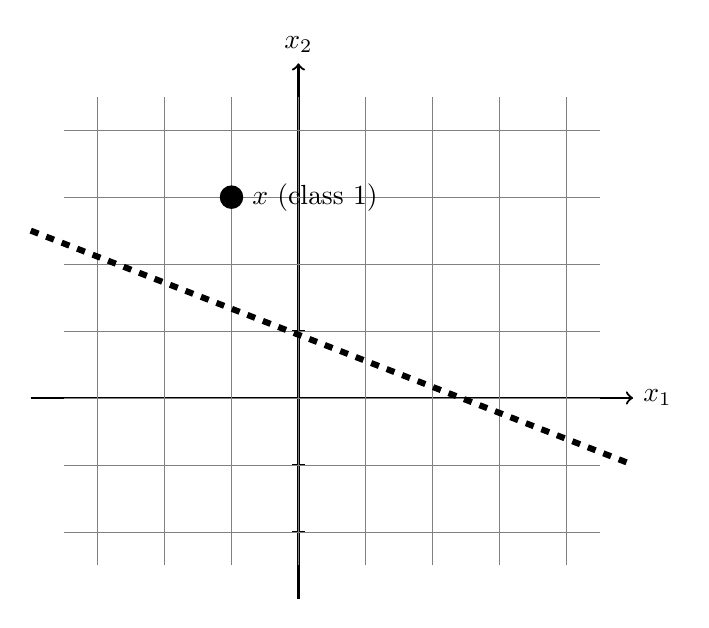
\begin{tikzpicture}[scale=0.85]
      \draw[->, thick] (-4, 0) -- (5, 0) node[right] {$x_1$};
      \draw[->, thick] (0, -3) -- (0, 5) node[above] {$x_2$};
      \foreach \t in {-3, ..., 4} \draw (\t, 0.1) -- (\t, -0.1);
      \foreach \t in {-2, ..., 4} \draw (0.1, \t) -- (-0.1, \t);
      \pick{%
        \draw[line width=2.2pt, dashed] (-2, -3) -- (3.5, 5);
        \fill (3, 1) circle (5pt) node[right=4pt] {$x$ (class 0)};}{%
        \draw[help lines, step=1] (-3.5, -2.5) grid (4.5, 4.5);
        \draw[line width=2.2pt, dashed] (-4, 2.5) -- (5, -1);
        \fill (-1, 3) circle (5pt) node[right=4pt] {$x$ (class 1)};}
    \end{tikzpicture}
  \end{center}

  \begin{enumerate}
    \item Give a weight vector $w$ and bias $b$ whose boundary is the dashed
      line and which put $x$ in its class.
    \item Is your $(w, b)$ the only one that works? Explain.
  \end{enumerate}
  \vfill
  \begin{center}3\end{center}
}{}

\end{document}
"
% \ver in {a, b} picks the version's numbers; \pg in {cover, q1, q2}.
\documentclass[11pt]{article}
\usepackage[letterpaper, margin=0.9in]{geometry}
\usepackage{amsmath, amssymb, booktabs, tikz, tcolorbox}
\usepackage{ifthen}
\usepackage[T1]{fontenc}
\usepackage{lmodern}
\pagestyle{empty}
\setlength{\parindent}{0pt}

\newcommand{\pick}[2]{\ifthenelse{\equal{\ver}{a}}{#1}{#2}}
\newcommand{\namebox}{%
  \begin{tcolorbox}[colback=gray!5!white, colframe=black!70!white,
      boxrule=0.6pt, sharp corners, left=8pt, right=8pt, top=10pt, bottom=10pt]
    \textbf{Name}: \makebox[2.8in]{\hrulefill}\hfill
    \textbf{Student ID}: \makebox[1.5in]{\hrulefill}
  \end{tcolorbox}}

\begin{document}

\ifthenelse{\equal{\pg}{cover}}{%
  DEMO 101 \hfill Example University\\
  Fall term \hfill Quiz 1
  \vspace{1.2in}
  \begin{center}
    {\Huge\bfseries Quiz 1}\\[10pt]
    {\Large Probability and linear classifiers}\\[4pt]
    {\large (fictional course, for the scan\_split example)}
  \end{center}
  \vspace{0.6in}
  \begin{tcolorbox}[colback=blue!4!white, colframe=blue!40!black,
      title={Instructions}]
    \begin{itemize}
      \item Write your name and student ID at the top of every question page.
      \item Keep all work for a question on that question's page; use its
        back if you need more room.
      \item Show your work; answers without work earn partial credit only.
      \item Calculators are allowed. No notes, no phones.
    \end{itemize}
  \end{tcolorbox}
  \vfill
  \begin{center}\large 20 minutes \quad$\cdot$\quad 20 points\end{center}
}{}

\ifthenelse{\equal{\pg}{q1}}{%
  \namebox
  \medskip
  \textbf{Problem 1 [10 pts] Which coin?}\par\smallskip
  A drawer holds two coins. Coin \pick{F}{G} is fair; coin
  \pick{L}{H} is loaded and lands heads with probability
  \pick{$0.8$}{$0.7$}. You pick coin \pick{L}{H} with probability
  \pick{$0.4$}{$0.25$}, flip it \pick{three}{four} times, and record the
  number of heads $K$.

  \medskip
  \begin{center}
    \begin{tabular}{c c c}
      \toprule
      $k$ & $P(K=k \mid \text{fair})$ & $P(K=k \mid \text{loaded})$\\
      \midrule
      \pick{%
        0 & 0.125 & 0.008\\ 1 & 0.375 & 0.096\\
        2 & 0.375 & 0.384\\ 3 & 0.125 & 0.512\\}{%
        0 & 0.0625 & 0.0081\\ 1 & 0.2500 & 0.0756\\
        2 & 0.3750 & 0.2646\\ 3 & 0.2500 & 0.4116\\ 4 & 0.0625 & 0.2401\\}
      \bottomrule
    \end{tabular}
  \end{center}
  \medskip
  You see $K = \pick{2}{3}$ heads. What is the probability that you picked
  the loaded coin?
  \vfill
  \begin{center}2\end{center}
}{}

\ifthenelse{\equal{\pg}{q2}}{%
  \namebox
  \medskip
  \textbf{Problem 2 [10 pts] Draw the boundary}\par\smallskip
  The dashed line is the decision boundary we want from a linear classifier
  $\hat y = \mathbb{1}[w^\top x + b > 0]$. The plotted point
  $x = \pick{[3, 1]^\top}{[-1, 3]^\top}$ belongs to class
  \pick{0}{1}.

  \begin{center}
    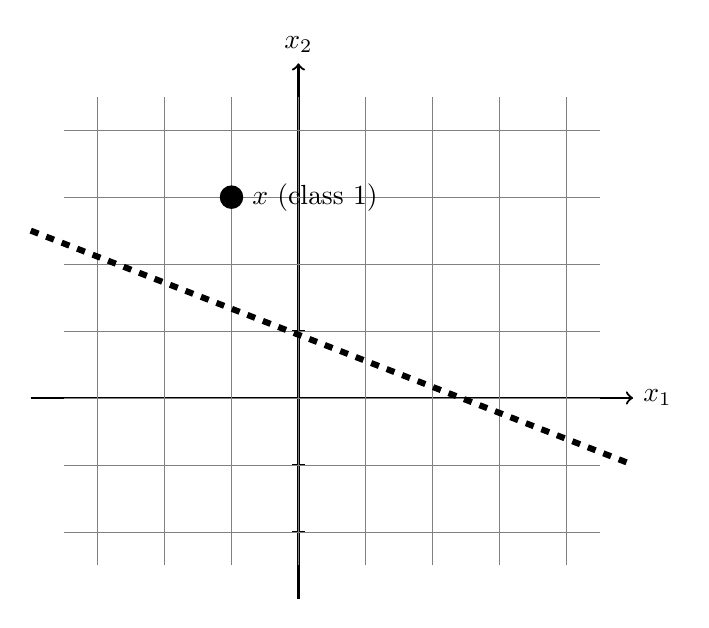
\begin{tikzpicture}[scale=0.85]
      \draw[->, thick] (-4, 0) -- (5, 0) node[right] {$x_1$};
      \draw[->, thick] (0, -3) -- (0, 5) node[above] {$x_2$};
      \foreach \t in {-3, ..., 4} \draw (\t, 0.1) -- (\t, -0.1);
      \foreach \t in {-2, ..., 4} \draw (0.1, \t) -- (-0.1, \t);
      \pick{%
        \draw[line width=2.2pt, dashed] (-2, -3) -- (3.5, 5);
        \fill (3, 1) circle (5pt) node[right=4pt] {$x$ (class 0)};}{%
        \draw[help lines, step=1] (-3.5, -2.5) grid (4.5, 4.5);
        \draw[line width=2.2pt, dashed] (-4, 2.5) -- (5, -1);
        \fill (-1, 3) circle (5pt) node[right=4pt] {$x$ (class 1)};}
    \end{tikzpicture}
  \end{center}

  \begin{enumerate}
    \item Give a weight vector $w$ and bias $b$ whose boundary is the dashed
      line and which put $x$ in its class.
    \item Is your $(w, b)$ the only one that works? Explain.
  \end{enumerate}
  \vfill
  \begin{center}3\end{center}
}{}

\end{document}
"
% \ver in {a, b} picks the version's numbers; \pg in {cover, q1, q2}.
\documentclass[11pt]{article}
\usepackage[letterpaper, margin=0.9in]{geometry}
\usepackage{amsmath, amssymb, booktabs, tikz, tcolorbox}
\usepackage{ifthen}
\usepackage[T1]{fontenc}
\usepackage{lmodern}
\pagestyle{empty}
\setlength{\parindent}{0pt}

\newcommand{\pick}[2]{\ifthenelse{\equal{\ver}{a}}{#1}{#2}}
\newcommand{\namebox}{%
  \begin{tcolorbox}[colback=gray!5!white, colframe=black!70!white,
      boxrule=0.6pt, sharp corners, left=8pt, right=8pt, top=10pt, bottom=10pt]
    \textbf{Name}: \makebox[2.8in]{\hrulefill}\hfill
    \textbf{Student ID}: \makebox[1.5in]{\hrulefill}
  \end{tcolorbox}}

\begin{document}

\ifthenelse{\equal{\pg}{cover}}{%
  DEMO 101 \hfill Example University\\
  Fall term \hfill Quiz 1
  \vspace{1.2in}
  \begin{center}
    {\Huge\bfseries Quiz 1}\\[10pt]
    {\Large Probability and linear classifiers}\\[4pt]
    {\large (fictional course, for the scan\_split example)}
  \end{center}
  \vspace{0.6in}
  \begin{tcolorbox}[colback=blue!4!white, colframe=blue!40!black,
      title={Instructions}]
    \begin{itemize}
      \item Write your name and student ID at the top of every question page.
      \item Keep all work for a question on that question's page; use its
        back if you need more room.
      \item Show your work; answers without work earn partial credit only.
      \item Calculators are allowed. No notes, no phones.
    \end{itemize}
  \end{tcolorbox}
  \vfill
  \begin{center}\large 20 minutes \quad$\cdot$\quad 20 points\end{center}
}{}

\ifthenelse{\equal{\pg}{q1}}{%
  \namebox
  \medskip
  \textbf{Problem 1 [10 pts] Which coin?}\par\smallskip
  A drawer holds two coins. Coin \pick{F}{G} is fair; coin
  \pick{L}{H} is loaded and lands heads with probability
  \pick{$0.8$}{$0.7$}. You pick coin \pick{L}{H} with probability
  \pick{$0.4$}{$0.25$}, flip it \pick{three}{four} times, and record the
  number of heads $K$.

  \medskip
  \begin{center}
    \begin{tabular}{c c c}
      \toprule
      $k$ & $P(K=k \mid \text{fair})$ & $P(K=k \mid \text{loaded})$\\
      \midrule
      \pick{%
        0 & 0.125 & 0.008\\ 1 & 0.375 & 0.096\\
        2 & 0.375 & 0.384\\ 3 & 0.125 & 0.512\\}{%
        0 & 0.0625 & 0.0081\\ 1 & 0.2500 & 0.0756\\
        2 & 0.3750 & 0.2646\\ 3 & 0.2500 & 0.4116\\ 4 & 0.0625 & 0.2401\\}
      \bottomrule
    \end{tabular}
  \end{center}
  \medskip
  You see $K = \pick{2}{3}$ heads. What is the probability that you picked
  the loaded coin?
  \vfill
  \begin{center}2\end{center}
}{}

\ifthenelse{\equal{\pg}{q2}}{%
  \namebox
  \medskip
  \textbf{Problem 2 [10 pts] Draw the boundary}\par\smallskip
  The dashed line is the decision boundary we want from a linear classifier
  $\hat y = \mathbb{1}[w^\top x + b > 0]$. The plotted point
  $x = \pick{[3, 1]^\top}{[-1, 3]^\top}$ belongs to class
  \pick{0}{1}.

  \begin{center}
    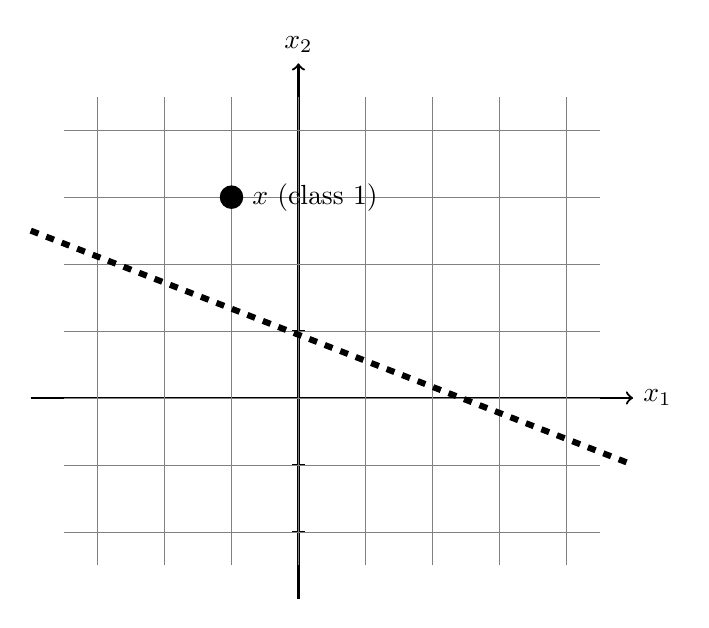
\begin{tikzpicture}[scale=0.85]
      \draw[->, thick] (-4, 0) -- (5, 0) node[right] {$x_1$};
      \draw[->, thick] (0, -3) -- (0, 5) node[above] {$x_2$};
      \foreach \t in {-3, ..., 4} \draw (\t, 0.1) -- (\t, -0.1);
      \foreach \t in {-2, ..., 4} \draw (0.1, \t) -- (-0.1, \t);
      \pick{%
        \draw[line width=2.2pt, dashed] (-2, -3) -- (3.5, 5);
        \fill (3, 1) circle (5pt) node[right=4pt] {$x$ (class 0)};}{%
        \draw[help lines, step=1] (-3.5, -2.5) grid (4.5, 4.5);
        \draw[line width=2.2pt, dashed] (-4, 2.5) -- (5, -1);
        \fill (-1, 3) circle (5pt) node[right=4pt] {$x$ (class 1)};}
    \end{tikzpicture}
  \end{center}

  \begin{enumerate}
    \item Give a weight vector $w$ and bias $b$ whose boundary is the dashed
      line and which put $x$ in its class.
    \item Is your $(w, b)$ the only one that works? Explain.
  \end{enumerate}
  \vfill
  \begin{center}3\end{center}
}{}

\end{document}
"
% \ver in {a, b} picks the version's numbers; \pg in {cover, q1, q2}.
\documentclass[11pt]{article}
\usepackage[letterpaper, margin=0.9in]{geometry}
\usepackage{amsmath, amssymb, booktabs, tikz, tcolorbox}
\usepackage{ifthen}
\usepackage[T1]{fontenc}
\usepackage{lmodern}
\pagestyle{empty}
\setlength{\parindent}{0pt}

\newcommand{\pick}[2]{\ifthenelse{\equal{\ver}{a}}{#1}{#2}}
\newcommand{\namebox}{%
  \begin{tcolorbox}[colback=gray!5!white, colframe=black!70!white,
      boxrule=0.6pt, sharp corners, left=8pt, right=8pt, top=10pt, bottom=10pt]
    \textbf{Name}: \makebox[2.8in]{\hrulefill}\hfill
    \textbf{Student ID}: \makebox[1.5in]{\hrulefill}
  \end{tcolorbox}}

\begin{document}

\ifthenelse{\equal{\pg}{cover}}{%
  DEMO 101 \hfill Example University\\
  Fall term \hfill Quiz 1
  \vspace{1.2in}
  \begin{center}
    {\Huge\bfseries Quiz 1}\\[10pt]
    {\Large Probability and linear classifiers}\\[4pt]
    {\large (fictional course, for the scan\_split example)}
  \end{center}
  \vspace{0.6in}
  \begin{tcolorbox}[colback=blue!4!white, colframe=blue!40!black,
      title={Instructions}]
    \begin{itemize}
      \item Write your name and student ID at the top of every question page.
      \item Keep all work for a question on that question's page; use its
        back if you need more room.
      \item Show your work; answers without work earn partial credit only.
      \item Calculators are allowed. No notes, no phones.
    \end{itemize}
  \end{tcolorbox}
  \vfill
  \begin{center}\large 20 minutes \quad$\cdot$\quad 20 points\end{center}
}{}

\ifthenelse{\equal{\pg}{q1}}{%
  \namebox
  \medskip
  \textbf{Problem 1 [10 pts] Which coin?}\par\smallskip
  A drawer holds two coins. Coin \pick{F}{G} is fair; coin
  \pick{L}{H} is loaded and lands heads with probability
  \pick{$0.8$}{$0.7$}. You pick coin \pick{L}{H} with probability
  \pick{$0.4$}{$0.25$}, flip it \pick{three}{four} times, and record the
  number of heads $K$.

  \medskip
  \begin{center}
    \begin{tabular}{c c c}
      \toprule
      $k$ & $P(K=k \mid \text{fair})$ & $P(K=k \mid \text{loaded})$\\
      \midrule
      \pick{%
        0 & 0.125 & 0.008\\ 1 & 0.375 & 0.096\\
        2 & 0.375 & 0.384\\ 3 & 0.125 & 0.512\\}{%
        0 & 0.0625 & 0.0081\\ 1 & 0.2500 & 0.0756\\
        2 & 0.3750 & 0.2646\\ 3 & 0.2500 & 0.4116\\ 4 & 0.0625 & 0.2401\\}
      \bottomrule
    \end{tabular}
  \end{center}
  \medskip
  You see $K = \pick{2}{3}$ heads. What is the probability that you picked
  the loaded coin?
  \vfill
  \begin{center}2\end{center}
}{}

\ifthenelse{\equal{\pg}{q2}}{%
  \namebox
  \medskip
  \textbf{Problem 2 [10 pts] Draw the boundary}\par\smallskip
  The dashed line is the decision boundary we want from a linear classifier
  $\hat y = \mathbb{1}[w^\top x + b > 0]$. The plotted point
  $x = \pick{[3, 1]^\top}{[-1, 3]^\top}$ belongs to class
  \pick{0}{1}.

  \begin{center}
    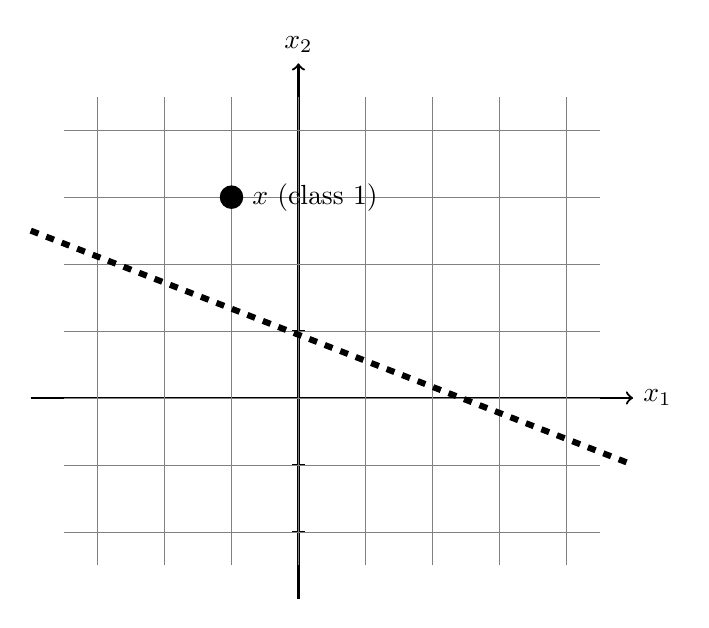
\begin{tikzpicture}[scale=0.85]
      \draw[->, thick] (-4, 0) -- (5, 0) node[right] {$x_1$};
      \draw[->, thick] (0, -3) -- (0, 5) node[above] {$x_2$};
      \foreach \t in {-3, ..., 4} \draw (\t, 0.1) -- (\t, -0.1);
      \foreach \t in {-2, ..., 4} \draw (0.1, \t) -- (-0.1, \t);
      \pick{%
        \draw[line width=2.2pt, dashed] (-2, -3) -- (3.5, 5);
        \fill (3, 1) circle (5pt) node[right=4pt] {$x$ (class 0)};}{%
        \draw[help lines, step=1] (-3.5, -2.5) grid (4.5, 4.5);
        \draw[line width=2.2pt, dashed] (-4, 2.5) -- (5, -1);
        \fill (-1, 3) circle (5pt) node[right=4pt] {$x$ (class 1)};}
    \end{tikzpicture}
  \end{center}

  \begin{enumerate}
    \item Give a weight vector $w$ and bias $b$ whose boundary is the dashed
      line and which put $x$ in its class.
    \item Is your $(w, b)$ the only one that works? Explain.
  \end{enumerate}
  \vfill
  \begin{center}3\end{center}
}{}

\end{document}
